% GNUPLOT: LaTeX picture with Postscript
\begingroup
  \makeatletter
  \providecommand\color[2][]{%
    \GenericError{(gnuplot) \space\space\space\@spaces}{%
      Package color not loaded in conjunction with
      terminal option `colourtext'%
    }{See the gnuplot documentation for explanation.%
    }{Either use 'blacktext' in gnuplot or load the package
      color.sty in LaTeX.}%
    \renewcommand\color[2][]{}%
  }%
  \providecommand\includegraphics[2][]{%
    \GenericError{(gnuplot) \space\space\space\@spaces}{%
      Package graphicx or graphics not loaded%
    }{See the gnuplot documentation for explanation.%
    }{The gnuplot epslatex terminal needs graphicx.sty or graphics.sty.}%
    \renewcommand\includegraphics[2][]{}%
  }%
  \providecommand\rotatebox[2]{#2}%
  \@ifundefined{ifGPcolor}{%
    \newif\ifGPcolor
    \GPcolortrue
  }{}%
  \@ifundefined{ifGPblacktext}{%
    \newif\ifGPblacktext
    \GPblacktexttrue
  }{}%
  % define a \g@addto@macro without @ in the name:
  \let\gplgaddtomacro\g@addto@macro
  % define empty templates for all commands taking text:
  \gdef\gplbacktext{}%
  \gdef\gplfronttext{}%
  \makeatother
  \ifGPblacktext
    % no textcolor at all
    \def\colorrgb#1{}%
    \def\colorgray#1{}%
  \else
    % gray or color?
    \ifGPcolor
      \def\colorrgb#1{\color[rgb]{#1}}%
      \def\colorgray#1{\color[gray]{#1}}%
      \expandafter\def\csname LTw\endcsname{\color{white}}%
      \expandafter\def\csname LTb\endcsname{\color{black}}%
      \expandafter\def\csname LTa\endcsname{\color{black}}%
      \expandafter\def\csname LT0\endcsname{\color[rgb]{1,0,0}}%
      \expandafter\def\csname LT1\endcsname{\color[rgb]{0,1,0}}%
      \expandafter\def\csname LT2\endcsname{\color[rgb]{0,0,1}}%
      \expandafter\def\csname LT3\endcsname{\color[rgb]{1,0,1}}%
      \expandafter\def\csname LT4\endcsname{\color[rgb]{0,1,1}}%
      \expandafter\def\csname LT5\endcsname{\color[rgb]{1,1,0}}%
      \expandafter\def\csname LT6\endcsname{\color[rgb]{0,0,0}}%
      \expandafter\def\csname LT7\endcsname{\color[rgb]{1,0.3,0}}%
      \expandafter\def\csname LT8\endcsname{\color[rgb]{0.5,0.5,0.5}}%
    \else
      % gray
      \def\colorrgb#1{\color{black}}%
      \def\colorgray#1{\color[gray]{#1}}%
      \expandafter\def\csname LTw\endcsname{\color{white}}%
      \expandafter\def\csname LTb\endcsname{\color{black}}%
      \expandafter\def\csname LTa\endcsname{\color{black}}%
      \expandafter\def\csname LT0\endcsname{\color{black}}%
      \expandafter\def\csname LT1\endcsname{\color{black}}%
      \expandafter\def\csname LT2\endcsname{\color{black}}%
      \expandafter\def\csname LT3\endcsname{\color{black}}%
      \expandafter\def\csname LT4\endcsname{\color{black}}%
      \expandafter\def\csname LT5\endcsname{\color{black}}%
      \expandafter\def\csname LT6\endcsname{\color{black}}%
      \expandafter\def\csname LT7\endcsname{\color{black}}%
      \expandafter\def\csname LT8\endcsname{\color{black}}%
    \fi
  \fi
    \setlength{\unitlength}{0.0500bp}%
    \ifx\gptboxheight\undefined%
      \newlength{\gptboxheight}%
      \newlength{\gptboxwidth}%
      \newsavebox{\gptboxtext}%
    \fi%
    \setlength{\fboxrule}{0.5pt}%
    \setlength{\fboxsep}{1pt}%
\begin{picture}(10800.00,7560.00)%
    \gplgaddtomacro\gplbacktext{%
      \csname LTb\endcsname%%
      \put(870,680){\makebox(0,0)[r]{\strut{}0}}%
      \csname LTb\endcsname%%
      \put(870,1197){\makebox(0,0)[r]{\strut{}10}}%
      \csname LTb\endcsname%%
      \put(870,1713){\makebox(0,0)[r]{\strut{}20}}%
      \csname LTb\endcsname%%
      \put(870,2230){\makebox(0,0)[r]{\strut{}30}}%
      \csname LTb\endcsname%%
      \put(870,2747){\makebox(0,0)[r]{\strut{}40}}%
      \csname LTb\endcsname%%
      \put(870,3263){\makebox(0,0)[r]{\strut{}50}}%
      \csname LTb\endcsname%%
      \put(972,494){\makebox(0,0){\strut{}0.07}}%
      \csname LTb\endcsname%%
      \put(2576,494){\makebox(0,0){\strut{}0.075}}%
      \csname LTb\endcsname%%
      \put(4180,494){\makebox(0,0){\strut{}0.08}}%
      \csname LTb\endcsname%%
      \put(5784,494){\makebox(0,0){\strut{}0.085}}%
      \csname LTb\endcsname%%
      \put(7387,494){\makebox(0,0){\strut{}0.09}}%
      \csname LTb\endcsname%%
      \put(8991,494){\makebox(0,0){\strut{}0.095}}%
      \csname LTb\endcsname%%
      \put(10595,494){\makebox(0,0){\strut{}0.1}}%
    }%
    \gplgaddtomacro\gplfronttext{%
      \csname LTb\endcsname%%
      \put(480,2230){\rotatebox{-270}{\makebox(0,0){\strut{}$\Delta \chi^2 - \Delta \chi^2_0$}}}%
      \csname LTb\endcsname%%
      \put(5783,215){\makebox(0,0){\strut{}$\sin^2 2 \theta_{13}$}}%
      \csname LTb\endcsname%%
      \put(6656,2654){\makebox(0,0){\strut{}Difference}}%
      \csname LTb\endcsname%%
      \put(6183,2468){\makebox(0,0)[l]{\strut{}$1\%$}}%
      \csname LTb\endcsname%%
      \put(6183,2282){\makebox(0,0)[l]{\strut{}$2\%$}}%
      \csname LTb\endcsname%%
      \put(6183,2096){\makebox(0,0)[l]{\strut{}$3\%$}}%
      \csname LTb\endcsname%%
      \put(6183,1910){\makebox(0,0)[l]{\strut{}$4\%$}}%
      \csname LTb\endcsname%%
      \put(6183,1724){\makebox(0,0)[l]{\strut{}$5\%$}}%
    }%
    \gplgaddtomacro\gplbacktext{%
      \csname LTb\endcsname%%
      \put(870,3780){\makebox(0,0)[r]{\strut{}0}}%
      \csname LTb\endcsname%%
      \put(870,4241){\makebox(0,0)[r]{\strut{}10}}%
      \csname LTb\endcsname%%
      \put(870,4702){\makebox(0,0)[r]{\strut{}20}}%
      \csname LTb\endcsname%%
      \put(870,5162){\makebox(0,0)[r]{\strut{}30}}%
      \csname LTb\endcsname%%
      \put(870,5623){\makebox(0,0)[r]{\strut{}40}}%
      \csname LTb\endcsname%%
      \put(870,6084){\makebox(0,0)[r]{\strut{}50}}%
      \csname LTb\endcsname%%
      \put(870,6545){\makebox(0,0)[r]{\strut{}60}}%
      \csname LTb\endcsname%%
      \put(870,7005){\makebox(0,0)[r]{\strut{}70}}%
      \csname LTb\endcsname%%
      \put(870,7466){\makebox(0,0)[r]{\strut{}80}}%
      \csname LTb\endcsname%%
      \put(972,3594){\makebox(0,0){\strut{}}}%
      \csname LTb\endcsname%%
      \put(2576,3594){\makebox(0,0){\strut{}}}%
      \csname LTb\endcsname%%
      \put(4180,3594){\makebox(0,0){\strut{}}}%
      \csname LTb\endcsname%%
      \put(5784,3594){\makebox(0,0){\strut{}}}%
      \csname LTb\endcsname%%
      \put(7387,3594){\makebox(0,0){\strut{}}}%
      \csname LTb\endcsname%%
      \put(8991,3594){\makebox(0,0){\strut{}}}%
      \csname LTb\endcsname%%
      \put(10595,3594){\makebox(0,0){\strut{}}}%
    }%
    \gplgaddtomacro\gplfronttext{%
      \csname LTb\endcsname%%
      \put(480,5623){\rotatebox{-270}{\makebox(0,0){\strut{}$\Delta \chi^2$}}}%
      \csname LTb\endcsname%%
      \put(5783,3538){\makebox(0,0){\strut{}}}%
      \csname LTb\endcsname%%
      \put(6656,7004){\makebox(0,0){\strut{}}}%
      \csname LTb\endcsname%%
      \put(6183,7004){\makebox(0,0)[l]{\strut{}No syst}}%
      \csname LTb\endcsname%%
      \put(6183,6818){\makebox(0,0)[l]{\strut{}$1\%$}}%
      \csname LTb\endcsname%%
      \put(6183,6632){\makebox(0,0)[l]{\strut{}$2\%$}}%
      \csname LTb\endcsname%%
      \put(6183,6446){\makebox(0,0)[l]{\strut{}$3\%$}}%
      \csname LTb\endcsname%%
      \put(6183,6260){\makebox(0,0)[l]{\strut{}$4\%$}}%
      \csname LTb\endcsname%%
      \put(6183,6074){\makebox(0,0)[l]{\strut{}$5\%$}}%
    }%
    \gplbacktext
    \put(0,0){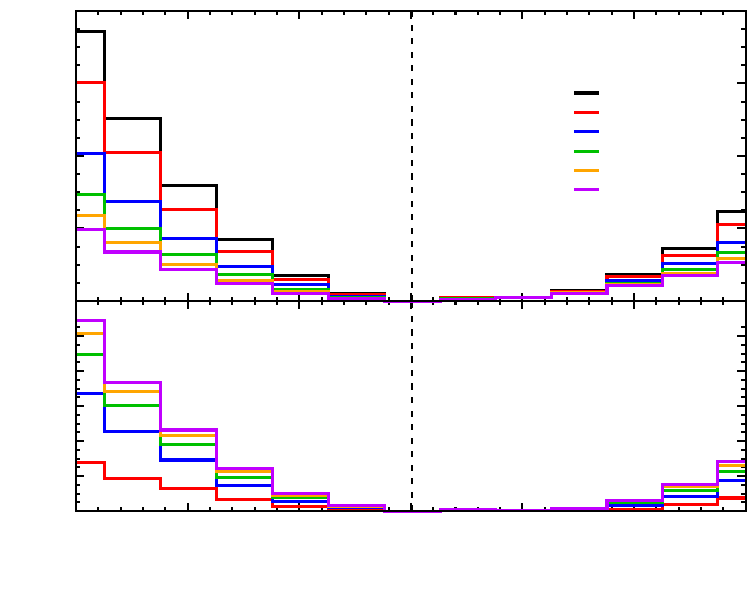
\includegraphics{nuenorm_corr_chi2_S13}}%
    \gplfronttext
  \end{picture}%
\endgroup
